\section{پیش بینی خطا}
\label{sec:bug-predict}
در این قسمت ابتدا نحوه‌ی پیش‌بینی خطا به طور کلی شرح داده می‌شود. سپس معیارهای متداول جهت ارزیابی مدل‌های پیش‌بینی بررسی می‌شوند. همانطور که اشاره شد جهت پیش‌بینی لازم است   معیارهایی از کد استخراج شود این معیارها به دو دسته‌ی کلی معیارهای کد و معیارهای فرآیند تقسیم می‌گردند. معیارهای مختلف معرفی شده در پژوهش‌های پیشین بررسی می‌شوند. در انتها   مدل‌هایی که جهت پیش‌بینی استفاده می‌گردد بازبینی می‌شوند. 

\subsection{فرآیند پیش‌بینی خطا}
\label{subsec:process}
اکثریت پژوهش‌های پیش‌بینی خطا از روش‌های یادگیری ماشین  استفاده کرده‌اند. اولین گام در ساخت مدل پیش‌بینی تولید داده‌هایی با استفاده از آرشیو‌های نرم‌افزاری همانند \واژه[سامانه‌های کنترل نسخه]{سامانه‌ی کنترل نسخه} مانند \نام{گیت}{Git}، سیستم‌های ردگیری مشکلات  مانند \نام{جیرا}{Jira} و آرشیو ایمیل‌ها است. هر یک از این داده‌ها بر اساس درشت دانگی پیش‌بینی می‌توانند نمایانگر یک سیستم، یک \واژه[قطعه‌ی]{قطعه} نرم‌افزاری، \واژه{بسته}، فایل کد منبع، کلاس و یا تابع باشد. مقصود از داده یک بردار ویژگی حاوی چندین معیار (یا ویژگی) می‌باشد که از آرشیو‌های نرم‌افزاری استخراج شده و دارای برچسب \موکد{سالم} و  \موکد{خطادار}  و یا تعداد خطاها است. پس از تولید داده‌ها با استفاده از معیارها و برچسب‌ها می‌توان به پیش پردازش داده‌ها پرداخت  که البته این امر اختیاری می‌باشد. پس از بدست آوردن مجموعه‌ی نهایی داده‌ها یک مدل پیش‌بینی را آموزش می‌دهیم که می‌تواند پیش‌بینی کند یک داده‌ی جدید حاوی خطا است یا خیر. تشخیص \واژه[خطاخیز]{خطا‌خیزی} بودن داده معادل \واژه{دسته‌بندی دوتایی}. مقصود از دسته‌بندی دوتایی، دسته‌بندی عناصر مجموعه‌ی داده شده به دو گروه مجزا می‌باشد. همچنین پیش‌بینی تعداد خطاها معادل \واژه{رگرسیون} می‌باشد.  منظور از رگرسیون فرآیند آماری است که در آن با استفاده از متغیرهای مستقل سعی می‌شود متغیر وابسته تخمین زده شود که در اینجا متغیرهای مستقل معیارهای پیش‌بینی خطا و متغیر وابسته تعداد خطاها می‌باشد. 

در شکل \ref{fig:prediction-process} فرآیند پیش‌بینی خطا نشان داده شده است. داده‌ها نمونه‌هایی هستند که می‌توانند خطادار  و بدون  خطا  بودن(   \lr{B = buggy} یا   \lr{C = clean} ) و یا تعداد خطا را نشان دهند. لازم به ذکر است که در یک مدل پیش‌بینی تنها از یک نوع از این داده‌ها استفاده می‌شود.
\begin{figure}[H]
	\centering
	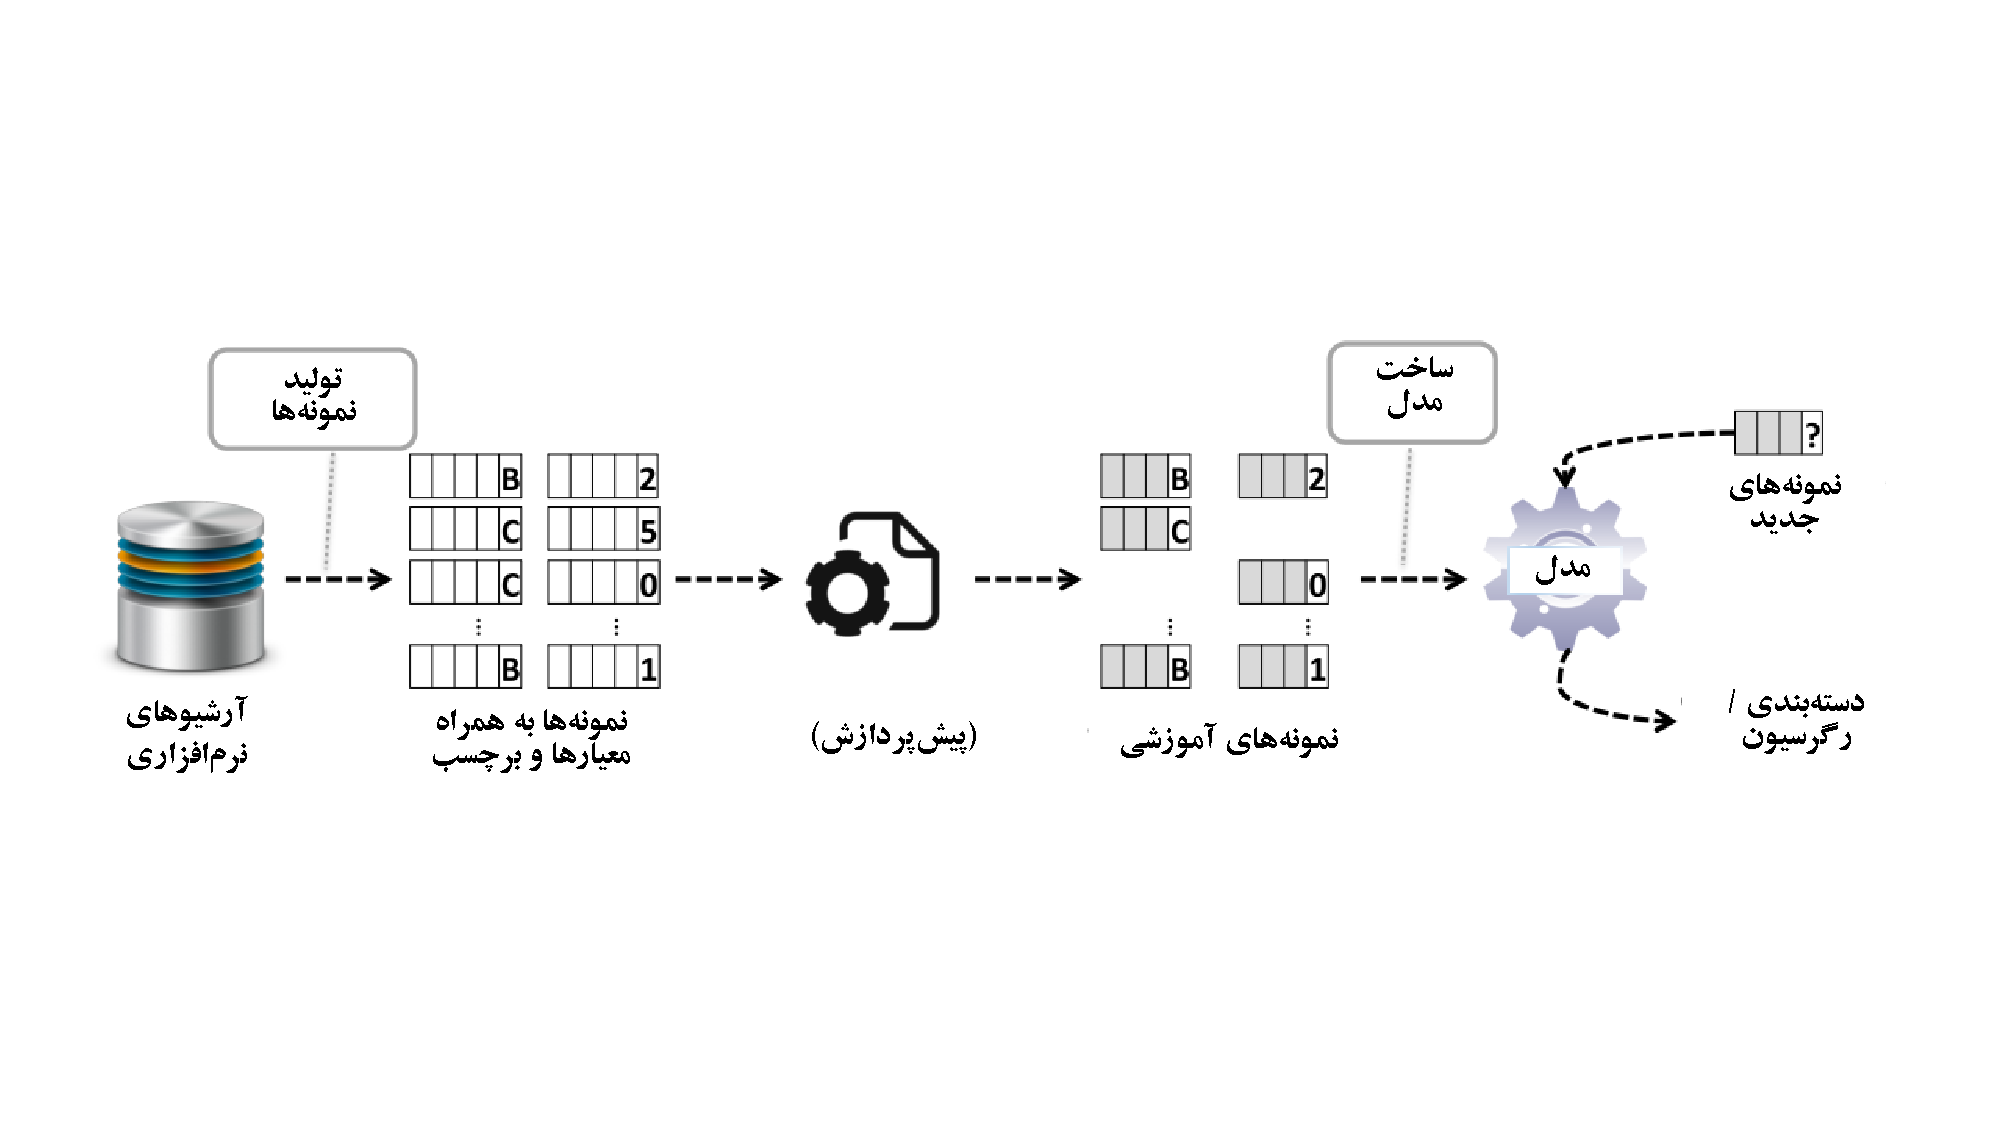
\includegraphics[trim={2cm 5cm 2cm 5cm},clip,width=1.0\textwidth]{img/prediction-process.pdf}
	 \caption{فرآیند پیش‌بینی خطا \cite{nam2014survey}}
	\label{fig:prediction-process}
\end{figure}